\section{Conceptual Design}

\subsection{Variations to the Requirement Analysis}
We modified the HW1 \lq\lq Requirement Analysis\rq\rq\ according to the feedback given during the evaluation. Specifically, we add to the \lq\lq Non-Functional Requirements\rq\rq\ section the privacy aspects that must be preserved while dealing with medical information.

\subsection{Entity-Relationship Schema}
Figure 1 shows the entity-relationship schema.
\begin{figure}[htp]
    \centering
    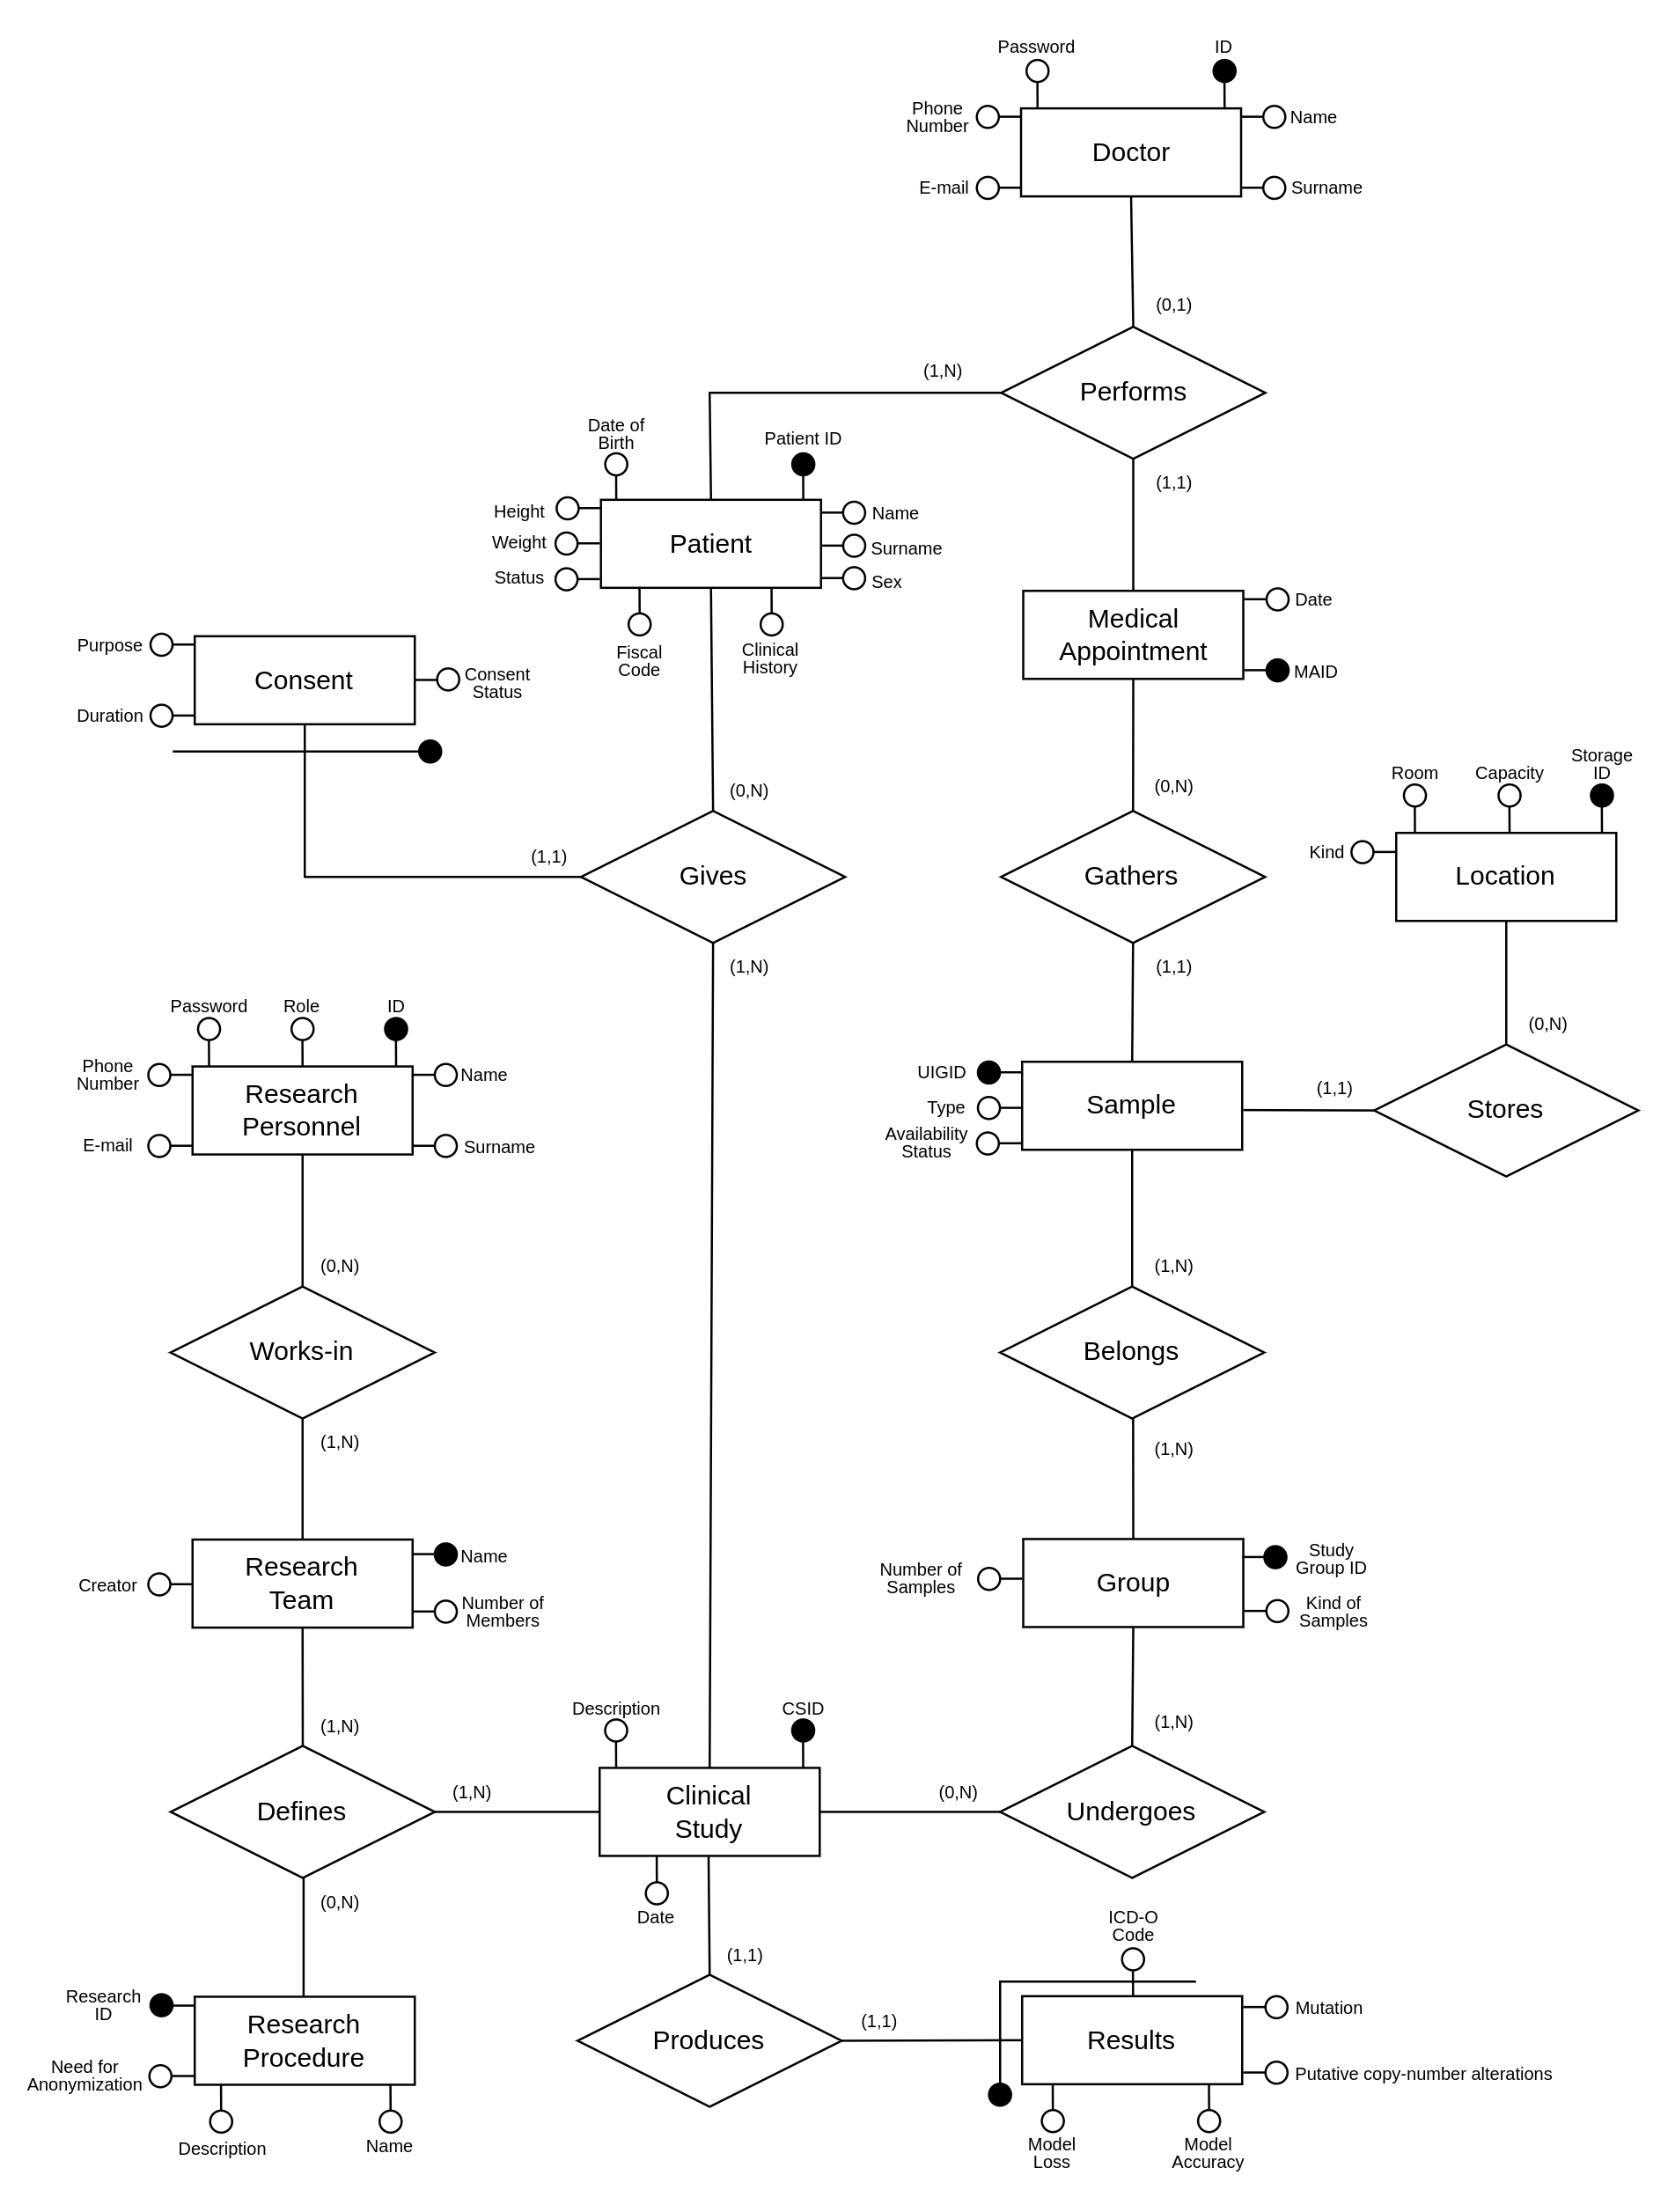
\includegraphics[width = 0.64\textwidth]{src/schemas/er_schema.png}
    \caption{Entity-Relationship Schema.}
\end{figure}

\subsection{Data Dictionary}

\subsubsection{Entities Table}
\begin{longtable}{|p{.20\columnwidth}|p{.20\columnwidth} |p{.30\columnwidth}|p{.25\columnwidth} |} 
\hline
\textbf{Entity} & \textbf{Description} & \textbf{Attributes} & \textbf{Identifier}  \\\hline


Clinical Study & Research study performed on samples, conducted by RHO’s Research Team (Data Scientists and Clinical Engineers). & \begin{itemize}
        \vspace{-1em}
        \item CSID (Clinical Study ID): identifier of the Clinical Study. (text)
        \item Date: the date on which the Clinical Study has been performed. (date range)
        \item Description: a brief explanation of the study's objectives and main features. (text)
        \end{itemize}
 &  CSID\\\hline
 
Consent & The consent the patient must provide during the medical appointment, according to the directives of the GDPR, for processing her/his data, which would then be involved in Clinical Studies if such consent is given. & \begin{itemize}
        \vspace{-1em}
        \item Consent Status: tells whether the patient has given the Consent for her/his data to be processed or not. (boolean)
        \item Duration: the period of time for which the Consent provided by the patient is maintained. (date range)
        \item Purpose: the reason why the patient is asked for Consent. (text)        
    \end{itemize}
 &  \begin{itemize}
    \vspace{-1em}
    \item Patient ID (from Patient)
    \item CSID (from Clinical Study)
 \end{itemize}
    \\\hline

Doctor & Medical employee of the RHO, responsible for performing medical examinations on patients, registering their data, and taking care of their medical treatment. & \begin{itemize}
        \vspace{-1em}
        \item ID: identifier of the Doctor. (text)
        \item E-mail: the e-mail address of the Doctor. (text)
        \item Name: the name of the Doctor. (text)
        \item Password: the login hashed password of the Doctor. (text)
        \item Phone Number: the phone number of the Doctor. (text)
        \item Surname: the surname of the Doctor. (text)
    \end{itemize}
 &  ID\\\hline

Group & The group to which each Sample can belong. & \begin{itemize}
        \vspace{-1em}
        \item Study Group ID: identifier of the Group to which the Sample belongs. (text)
        \item Kind of Samples: the type of Sample collected, e.g., blood samples, tissues, genome type. (text)
        \item Number of Samples: the number of samples that a Group contains. (integer)
    \end{itemize}
 &  Study Group ID\\\hline

Location & The physical location in which each Sample is stored. & \begin{itemize}
        \vspace{-1em}
        \item Storage ID: identifier of the Location where the sample is stored. (text)
        \item Capacity: the number of samples each Location can contain. (integer)
        \item Kind: the type of sample storage Location, e.g., refrigerator and boxes. (text)
        \item Room: the room where samples can be stored. (text)
    \end{itemize}
 &  Storage ID\\\hline

Medical Appointment & The medical examination that a doctor performs on a patient. Thanks to it, the doctor can enter and/or update patient information and (if necessary) collect one or more biological samples for further analysis. & \begin{itemize}
        \vspace{-1em}
        \item MAID (Medical Appointment ID): identifier of the Medical Appointment. (text)
        \item Date: the date on which the Medical Appointment has been performed. (date range)
    \end{itemize}
 &  MAID\\\hline

Patient & Person who undergoes a medical examination at the RHO Institute to receive a diagnosis and (if necessary) a treatment for her/his oncological pathology. In addition, the patient should consent for the RHO's researchers to study his/her biological samples. & \begin{itemize}
        \vspace{-1em}
        \item Patient ID: identifier of the Patient. (serial)
        \item Clinical History: a description of the clinical history (medical appointments, treatments) of the Patient. (text)
        \item Date of Birth: the date of birth of the Patient. (date range)
        \item Fiscal Code: the fiscal code of the Patient. (text)
        \item Height: the height of the Patient. (float)
        \item Name: the name of the Patient. (text)
        \item Sex: the sex of the Patient. (text)
        \item Status: identifies whether the Patient is sick or healthy. (boolean)
        \item Surname: the surname of the Patient. (text)
        \item Weight: the weight of the Patient. (float)
    \end{itemize}
 &  Patient ID\\\hline

Research Personnel & Entity that groups all the RHO researchers (Clinical Engineers and Data Scientists) involved in research activities and analyses. & \begin{itemize}
        \vspace{-1em}
        \item ID: identifier of the Research Personnel member. (text)
        \item E-mail: the e-mail address of the Research Personnel member. (text)
        \item Name: the name of the Research Personnel member. (text)
        \item Password: the log-in hashed password of the Research Personnel member. (text)
        \item Phone Number: the phone number of the Research Personnel member. (text)
        \item Role: identifies whether the researcher is a Clinical Engineer or a Data Scientist. (boolean)
        \item Surname: the surname of the Research Personnel member. (text)
    \end{itemize}
 &  ID\\\hline

Research Procedure & The statistical and/or biochemical methodology that Clinical Engineers and Data Scientists use to conduct a Clinical Study. & \begin{itemize}
        \vspace{-1em}
        \item Research ID: identifier of the Research Procedure. (text)
        \item Description: a brief explanation of the objectives and the main features of the Research Procedure. (text)
        \item Name: identifier of the Procedure adopted. (text)
        \item Need for Anonymization: identifies whether the Research Procedure used has to be anonymized or not. (boolean)
    \end{itemize}
 &  Research ID\\\hline

Research Team & A group of researchers, composed of Clinical Engineers and Data Scientists, that performs the analyses required by a Clinical Study. & \begin{itemize}
        \vspace{-1em}
        \item Name: identifier of the Research Team. (text)
        \item Creator: the researcher who created the Research Team. (text)
        \item Number of Members: the number of members of the Research Team. (integer)
    \end{itemize}
 &  Name\\\hline

Results & The set of statistical and biochemical results obtained at the end of a Clinical Study. & \begin{itemize}
        \vspace{-1em}
        \item ICD-O Code: identifier of the Results obtained. (text)
        \item Model Accuracy: the value of the accuracy metric that describes the performance of the statistical model used. (float)
        \item Model Loss: the value of the loss metric for the statistical model used. (float)
        \item Mutation: number of mutations discovered. (integer)
        \item Putative copy-number alterations: a measure of genomic instability. (float)
    \end{itemize}
 &  \begin{itemize}
    \vspace{-1em}
    \item ICD-O Code
    \item CSID (from Clinical Study)
 \end{itemize}
    \\\hline

Sample & A biochemical sample, e.g., blood, tissue, or genome, that a doctor collects from a patient during a medical appointment and that will be analyzed in a Clinical Study together with its Group. & \begin{itemize}
        \vspace{-1em}
        \item UIGID (Unique Incrementally Generated ID): identifier of the Sample. (serial)
        \item Availability Status: identifies whether the Sample is available or not. (boolean)
        \item Type: the type of the Sample. (text)
    \end{itemize}
 &  UIGID\\\hline
 
\end{longtable}


\subsubsection{Relationships Table}
\begin{longtable}{|p{.20\columnwidth}|p{.20\columnwidth} |p{.30\columnwidth}|p{.25\columnwidth} |}
\hline
\textbf{Relationship} & \textbf{Description} & \textbf{Component Entities} & \textbf{Attributes} \\\hline


Belongs & It associates a collected Sample with the Group to which it belongs. & \begin{itemize}
        \vspace{-1em}
        \item Group (1, N).
        \item Sample (1, N).
    \end{itemize}
 &  --- \\\hline

 Defines & It associates a Research Team, the Clinical Study in which its members are involved, and the Research Procedure followed to perform it. & \begin{itemize}
        \vspace{-1em}
        \item Clinical Study (1, N).
        \item Research Procedure (0, N).
        \item Research Team (1, N).
    \end{itemize}
 &  --- \\\hline

 Gathers & It associates a biochemical Sample with the Medical Appointment, during which it could be collected from the patient for further analyses. & \begin{itemize}
        \vspace{-1em}
        \item Medical Appointment (0, N).
        \item Sample (1, 1).
    \end{itemize}
 &  --- \\\hline

 Gives & It associates the Patient with the Consent she/he could give for her/his data to be used in the relevant Clinical Study. & \begin{itemize}
        \vspace{-1em}
        \item Clinical Study (1, N)
        \item Consent (1, 1).
        \item Patient (0, N).
    \end{itemize}
 &  --- \\\hline

 Performs & It associates a Doctor with a Patient and the Medical Appointment that can be performed on her/him. & \begin{itemize}
        \vspace{-1em}
        \item Doctor (0, 1).
        \item Medical Appointment (1, 1).
        \item Patient (1, N).
    \end{itemize}
 &  --- \\\hline

 Produces & It associates a Clinical Study with the Results obtained from its procedures and analyses. & \begin{itemize}
        \vspace{-1em}
        \item Clinical Study (1, 1).
        \item Results (1, 1).
    \end{itemize}
 &  --- \\\hline

 Stores & It associates a collected Sample with the physical Location where it is stored. & \begin{itemize}
        \vspace{-1em}
        \item Location (0, N).
        \item Sample (1, 1).
    \end{itemize}
 &  --- \\\hline

 Undergoes & It associates a Group of samples with the Clinical Study in which they will be analyzed. & \begin{itemize}
        \vspace{-1em}
        \item Clinical Study (0, N).
        \item Group (1, N).
    \end{itemize}
 &  --- \\\hline

 Works-in & It associates the Research Personnel members with the Research Team in which they participate. & \begin{itemize}
        \vspace{-1em}
        \item Research Personnel (0, N).
        \item Research Team (1, N).
    \end{itemize}
 &  --- \\\hline

\end{longtable}


\subsection{External Constraints}
\begin{itemize}
    \item Each research team must comprise at least one clinical engineer and one data scientist from the research personnel.\\
    Moreover, the attribute 'Number of Members' of the 'Research Team' entity must be updated each time a new member gets added or removed from the group.
    \item A medical appointment can produce a sample only before having the consent form from the patient.
    \item The attribute 'Number of Samples' of the 'Group' entity must be updated each time a new sample gets added or removed from the group.
    \item A clinical study can be carried out insofar as it stays between the boundaries provided by the "Comitato Etico Unico Regionale" (CEUR) and not for other scopes.
\end{itemize}

\subsection{Functional Requirements Satisfaction Check}
Considering the Functional Requirements from HW1 and intending to improve the clarity of this section, we divide the data that the database must store into four categories of data, namely \textbf{Organizational}, \textbf{Patient}, \textbf{Personnel}, and \textbf{Research}.
\begin{itemize} 

    \item \textbf{Organizational} data, i.e., data related to the logistics aspects at the RHO Institute.

    Group of sample data, including:
    \begin{itemize}
        \item The kind of Samples in the group.
        \item The study Group ID.
    \end{itemize}
    Location of samples storing data, including:
    \begin{itemize}
        \item The capacity of the storing device.
        \item The storing device.
        \item The room where the sample is stored.
    \end{itemize}
    Medical appointment data, including:
    \begin{itemize}
        \item The date the medical appointment is performed.
    \end{itemize}
    Sample data, including:
    \begin{itemize}
        \item Biological data concerning the typology of the sample.
        \item The availability of the sample.
    \end{itemize}   
    Such information is stored in the \emph{Group}, \emph{Location}, \emph{Medical Appointment}, and \emph{Sample} entities, respectively. On the one hand, the \emph{Gathers} relationship defines the association between the medical appointment in which a sample is collected; on the other hand, the \emph{Stores} relationship keeps the information concerning where the samples are held. The relationship \emph{Belongs} defines the information about which sample is part of one or more Sample Groups.

    \item \textbf{Patient} data, i.e., data from individuals who arrive at the RHO Institute. 

    Consent data, including:
    \begin{itemize}
        \item Consensus status.
        \item Duration.
        \item Purpose.
    \end{itemize}
    Patient data, including:
    \begin{itemize}
        \item Clinical history.
        \item Date of birth.
        \item Fiscal code.
        \item Height.
        \item Name.
        \item Sex.
        \item Status.
        \item Surname.
        \item Weight.
    \end{itemize}
    Such information is stored in the \emph{Consent} and \emph{Patient} entities, respectively. The relationship \emph{Gives} links the consent to each patient and the respective Clinical Study.
    
    \item \textbf{Personnel} data, i.e., data connected to the individuals that work in the RHO Institute.

    Doctors data:
    \begin{itemize}
        \item Contact info (E-mail and phone number).
        \item Name.
        \item Surname.
        \item Hashed password for login.
    \end{itemize}
    Research personnel data:
    \begin{itemize}
        \item Contact info (E-mail and phone number).
        \item Name.
        \item Surname.
        \item Role.
        \item Hashed password for login.
    \end{itemize}
    Such information is stored in the \emph{Doctor} and \emph{Research Personnel} entities. In this case, there is a need for a distinction in the roles of the RHO employees since the Research personnel does not perform medical appointments or enroll patients in the systems, while the doctors do not define research procedures or create research teams. The relationship \emph{Performs} defines which medical appointment is related to which doctor.

    \item \textbf{Research} data, i.e., data related to the Oncological research aspects carried out in the RHO Institute.

    Clinical studies data:
    \begin{itemize}
        \item Description of the Oncological Research Study performed.
        \item The period of time on which the Clinical Study is performed.
    \end{itemize}
    Research procedures data:
    \begin{itemize}
        \item Name of the procedure adopted.
        \item Need for anonymization of the sensitive information used in the clinical study.
        \item Description and direction of the Research Pipeline.
    \end{itemize}
    Research team data:
    \begin{itemize}
        \item Creator of the Team.
        \item Name of the Team.
        \item Number of members in the Team.
    \end{itemize}
    Results data:
    \begin{itemize}
        \item Model statistics after the experiments.
        \item Number of mutations computed.
        \item Value of genomics instability obtained.
    \end{itemize}
    Such information is stored in \emph{Clinical Study}, \emph{Research Procedure}, \emph{Research Team}, and \emph{Results} entities, respectively. The relationship \emph{Works-in} defines the relations between the individual research employee and the Research team in which he/she works. Moreover, the relationship \emph{Produces} stores the information between the experiments and the results, i.e., the Clinical Studies and the results.
\end{itemize}

Moreover, the system must allow: 
\begin{itemize}
    \item \textbf{Doctors, Clinical Engineers, and Data Scientists to log in and sign up, managing different user roles for them.} The information is stored in the entities \emph{Doctor} and \emph{Research personnel} and the relationships \emph{Perform} and \emph{Works-in} allow the system to differentiate between the different roles.
    \item \textbf{Doctors to register and update patients' personal and medical information and perform medical appointments for each patient.} The information is stored in the entities \emph{Medical Appointment} and \emph{Patient}. The relationship \emph{Performs} allows the system to keep track of the information of the medical appointment performed on the patient.
    \item \textbf{Clinical Engineers to label and store samples.} The data is stored in the \emph{Location} and \emph{Sample} entities. The information is defined in the relationship \emph{Stores}.
    \item \textbf{Clinical Engineers perform clinical studies for each sample and update their biochemical data.} The information is available in the \emph{Results} produced by different Clinical Studies, via the relationship \emph{Produces}.
    \item \textbf{Data Scientist to access the biochemical and clinical data of the samples, updating statistical studies.} The data is stored in entity \emph{Results}, where the statistical information of the Clinical study is reported.
    \item \textbf{Researchers (Clinical Engineers and Data Scientists) to create/join a Research Team.} The relationship \emph{Works-in} allows the system to organize the distribution of the research teams. The data is stored in the \emph{Research Team} entity.
\end{itemize}